% Meta-Diffusion: the measurement package's results, in brief
%
% Compile:  pdflatex results_jinjian.tex
% Requires: amsmath amssymb booktabs enumitem xcolor graphicx tikz geometry hyperref
%
% Figure 1 is docs/figures/gen_grid.png, written by scripts/gen_specificity.py.
% Every number here came from handoff/Jinjian/results/ on 11 September 2026.

\documentclass[11pt]{article}

\usepackage[a4paper,margin=0.8in]{geometry}
\usepackage{amsmath,amssymb}
\usepackage{booktabs}
\usepackage{enumitem}
\usepackage{graphicx}
\usepackage{xcolor}
\usepackage{tikz}
\usepackage[font=small,labelfont=bf]{caption}
\usepackage{hyperref}

\definecolor{accent}{HTML}{7A2E4E}
\definecolor{sblue}{HTML}{2A78D6}
\definecolor{sorange}{HTML}{EB6834}
\definecolor{saqua}{HTML}{1BAF7A}
\definecolor{bad}{HTML}{A0392A}
\definecolor{rulegrey}{HTML}{CFC3C9}

\hypersetup{colorlinks=true, linkcolor=accent, urlcolor=accent}

\newcommand{\code}[1]{\texttt{\small #1}}
\newcommand{\KT}{K_{T}}
\newcommand{\dtask}{\Delta_{\mathrm{task}}}

\setlist[itemize]{leftmargin=1.3em, itemsep=2pt, topsep=2pt}
\pagestyle{empty}
\setlength{\emergencystretch}{3em}

\begin{document}

\begin{center}
{\Large\bfseries What the loss hid}\\[2pt]
{\small The task coordinate was written off on the strength of a denoising loss that
barely moves. In generated samples it decides the outcome every time.}\\[4pt]
{\footnotesize\ttfamily cifar\_ds3 @ 50k $\cdot$ validation $\cdot$ 24 episodes $\cdot$
128 samples per cell $\cdot$ DDIM $\eta=0$, 50 steps}
\end{center}

\vspace{2pt}
\noindent\rule{\textwidth}{0.8pt}
\vspace{4pt}

\noindent
\begin{minipage}[t]{0.31\textwidth}
{\Large\bfseries\color{accent} 100\,\%}\\[2pt]
{\footnotesize of generated sets carry the \textbf{right transformation} given the
episode's own coordinate --- against 33\,\% chance}
\end{minipage}\hfill
\begin{minipage}[t]{0.31\textwidth}
{\Large\bfseries 1.7\,\%}\\[2pt]
{\footnotesize is all the \textbf{same coordinate} is worth on the denoising loss the
project has been reading}
\end{minipage}\hfill
\begin{minipage}[t]{0.31\textwidth}
{\Large\bfseries\color{accent} 5.7$\times$}\\[2pt]
{\footnotesize closer to the target domain than reusing the source coordinate, at
$\KT = 1$}
\end{minipage}

\vspace{8pt}
\noindent\rule{\textwidth}{0.4pt}

\vspace{-6pt}
\section*{The picture without any instrument}

\begin{figure}[!ht]
\centering

\includegraphics[width=0.80\textwidth]{figures/gen_grid.png}
\caption{Each column starts from \textbf{one shared initial noise}, so composition is
fixed down the column and only the coordinate changes. Columns 1--6 are blur tasks,
7--8 noise tasks. The \code{own} row follows the task; \code{mean} and \code{zero}
ignore it; \code{shuffled} follows the \emph{wrong} task.}
\end{figure}

\begin{figure}[!ht]
\centering
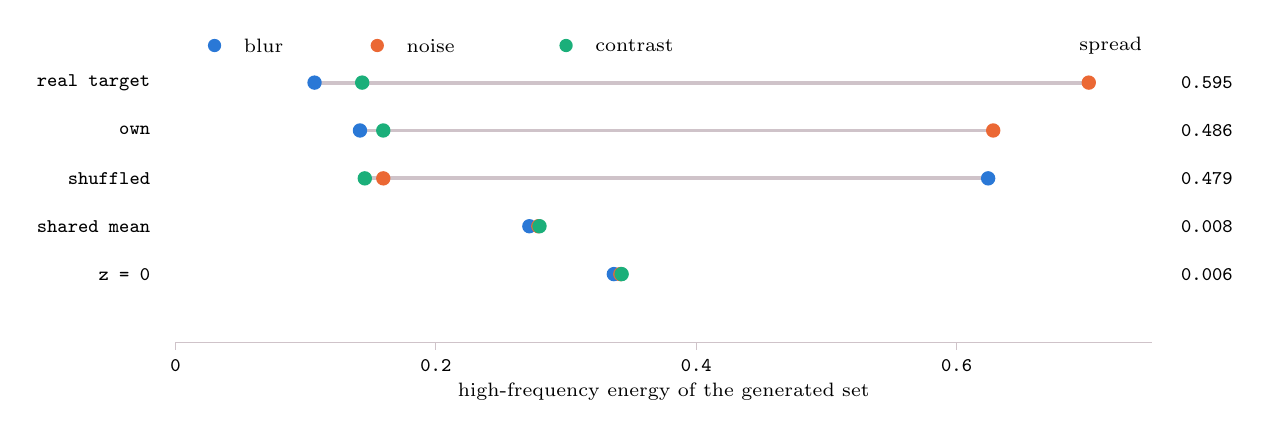
\begin{tikzpicture}[x=12.4cm/0.75, y=0.76cm]
  % axis
  \draw[rulegrey] (0,-0.35) -- (0.75,-0.35);
  \foreach \v in {0,0.2,0.4,0.6}{
    \draw[rulegrey] (\v,-0.35) -- (\v,-0.47);
    \node[below,font=\scriptsize\ttfamily] at (\v,-0.47) {\v};
  }
  \node[below,font=\scriptsize] at (0.375,-0.85)
    {high-frequency energy of the generated set};

  % legend
  \fill[sblue]   (0.03,4.62) circle (2.4pt); \node[right,font=\scriptsize] at (0.045,4.62) {blur};
  \fill[sorange] (0.155,4.62) circle (2.4pt); \node[right,font=\scriptsize] at (0.17,4.62) {noise};
  \fill[saqua]   (0.30,4.62) circle (2.4pt); \node[right,font=\scriptsize] at (0.315,4.62) {contrast};
  \node[left,font=\scriptsize] at (0.75,4.62) {spread};

  % rows: name, y, blur, noise, contrast, spread
  \foreach \nm/\y/\b/\n/\c/\s in {%
    real target/4.0/0.1068/0.7015/0.1434/0.595,
    own/3.2/0.1417/0.6281/0.1596/0.486,
    shuffled/2.4/0.6242/0.1596/0.1454/0.479,
    shared mean/1.6/0.2718/0.2787/0.2796/0.008,
    z = 0/0.8/0.3367/0.3417/0.3427/0.006}{
      \node[left,font=\scriptsize\ttfamily] at (-0.012,\y) {\nm};
      \pgfmathsetmacro{\lo}{min(\b,min(\n,\c))}
      \pgfmathsetmacro{\hi}{max(\b,max(\n,\c))}
      \draw[rulegrey,line width=1.4pt] (\lo,\y) -- (\hi,\y);
      \fill[sblue]   (\b,\y) circle (2.6pt);
      \fill[sorange] (\n,\y) circle (2.6pt);
      \fill[saqua]   (\c,\y) circle (2.6pt);
      \node[right,font=\scriptsize\ttfamily] at (0.765,\y) {\s};
  }
\end{tikzpicture}
\caption{Blur suppresses high-frequency energy, added noise raises it. A coordinate that
carries the task spreads its three values apart. \code{own} reproduces 82\,\% of the real
spread; \code{mean} and \code{zero} collapse onto a point; \code{shuffled} spreads just
as far, in the wrong direction --- which is what rules out every explanation that does
not run through the coordinate.}
\end{figure}

\section*{Deployment strategies, re-run in this metric}

\noindent Distance from the real target domain, lower is better. The denoising loss puts
all six rows on the same number.

\vspace{4pt}
\noindent
\begin{tabular}{@{}lrrr@{}}
\toprule
strategy & $\KT = 1$ & $\KT = 5$ & $\KT = 20$ \\
\midrule
no adaptation            & 1.577 & 1.614 & 1.607 \\
reuse $z_S$              & 1.410 & 0.805 & 0.484 \\
\textbf{transport}       & \textbf{0.249} & \textbf{0.272} & \textbf{0.271} \\
transport + refine       & 0.245 & 0.300 & \textcolor{bad}{\textbf{0.356}} \\
target only              & 0.276 & 0.285 & 0.253 \\
oracle                   & 0.258 & 0.253 & 0.249 \\
\bottomrule
\end{tabular}

\vspace{8pt}
\begin{itemize}
  \item \textbf{Transport beats reusing the source coordinate} by $+1.161 \pm 0.233$ at
    $\KT = 1$, shrinking to $+0.213$ at $\KT = 20$ --- the shape the method predicts, and
    the shape stage 1 produced on Gaussian mixtures.
  \item \textbf{Transport does not beat encoding one target image} ($+0.027 \pm 0.096$).
    The transformation is too easy to read from a single sample for source information to
    add anything.
  \item \textbf{Refinement makes samples worse, and worse with more data}
    ($0.245 \to 0.300 \to 0.356$). It optimises the loss, and the loss is the thing that
    disagrees with the samples.
\end{itemize}

\section*{What this changes}

\begin{itemize}
  \item \textbf{The representation was never the problem.} The instrument that said so
    compresses the effect by roughly fifty-fold. The earlier ``0\,\% task-specific''
    result reproduces exactly on the arm it was measured on --- one transformation, 32
    channels --- and does not generalise to the arm where tasks differ in something
    denoising depends on.
  \item \textbf{Switch refinement off} in this setting, or re-point it at an objective
    that agrees with the samples.
  \item \textbf{The centring change is no longer the indicated fix.} It was the remedy
    for a representation with no task-specific content, and that diagnosis has not
    survived.
\end{itemize}

\section*{What these numbers do not say}

\begin{itemize}
  \item Nothing clean about \textbf{semantic class}: the coordinate carries
    transformation identity ($+0.00133 \pm 0.00035$, 98.5\,\% of the effect) and almost
    no class identity ($+0.00002 \pm 0.00001$, 1.5\,\%).
  \item Generation reaches \textbf{82\,\%} of the way to the target domain, not all of
    it --- and the oracle does no better, so the residual gap is the model's reach rather
    than a mis-set coordinate.
  \item Everything here is the \textbf{three-transformation checkpoint}. The
    single-transformation arms show $\dtask \approx 0$ and have not been put through the
    generation test.
\end{itemize}

\vfill
\noindent{\footnotesize\ttfamily branch jinjian $\cdot$ scripts/posthoc\_controls.py,
gen\_specificity.py, gen\_strategies.py $\cdot$ raw output in
handoff/Jinjian/results/}

\end{document}
